%%==============================================================
%% Shenzhen MSU-BIT University - Bachelor Thesis
%% 五连杆轮腿平衡机器人的运动仿真与控制研究与实现
%% 编译链: xelatex -> bibtex -> xelatex -> xelatex
%%==============================================================
\documentclass{smbuthesis}

% --- Thesis title (shown before main body) ---
\smbutitle{五连杆轮腿平衡机器人的运动仿真与控制研究与实现}

% --- Required packages ---
\usepackage{rotating}
\usepackage{multirow}
\usepackage{ragged2e}
\usepackage{array}
\usepackage{makecell}
\usepackage{textcomp}
\usepackage{booktabs}
\usepackage{amsfonts}
\usepackage{cite}
\usepackage{dblfloatfix}
\usepackage{placeins}
\usepackage{subcaption}
\usepackage{nicefrac}
\usepackage{fancyhdr}
\pagestyle{fancy}
\usepackage{amsmath}
\usepackage{float}
\usepackage{amssymb}
\usepackage[final]{pdfpages}
\usepackage{dsfont}
\usepackage{algorithm}
\usepackage{algorithmic}
\usepackage{graphicx}
\usepackage{cleveref}

%% 图片支持：SVG 需 Inkscape + --shell-escape；若环境无 Inkscape，
%% 请先把 figures/*.svg 转成同名 .pdf（rsvg-convert -f pdf in.svg > out.pdf
%% 或 inkscape in.svg --export-pdf=out.pdf），然后用 \includegraphics 即可。
\graphicspath{{figures/}}

% --- Custom commands ---
\DeclareMathOperator*{\argmin}{argmin}
\DeclareMathOperator{\Proj}{Proj}
\newcommand{\bragg}[1]{{\mbox{\bfseries BR-AGG}(#1)}}

% 占位图（图未到位时，先用同尺寸框占编号；后续替换为 \includegraphics 即可）
% 用法：\figplaceholder{说明文字}        — 高度 0.30\textwidth
%       \figplaceholder[0.45]{说明文字} — 自定义高度
\newcommand{\figplaceholder}[2][0.30]{%
  \fbox{\begin{minipage}[c][#1\textwidth][c]{0.92\textwidth}%
    \centering\itshape\small (占位图待补：#2)%
  \end{minipage}}%
}
\newtheorem{theorem}{\textbf{Theorem}}
\newtheorem{lemma}{\textbf{Lemma}}
\newtheorem{assump}{\textbf{Assumption}}
\newtheorem{remark}{\textbf{Remark}}
\newtheorem{definition}{\textbf{Definition}}
\newtheorem{proposition}{\textbf{Proposition}}

%%==============================================================

\begin{document}
\pagenumbering{arabic}
\setcounter{page}{1}
\pagestyle{fancy}

% --- 封面 PDF ---
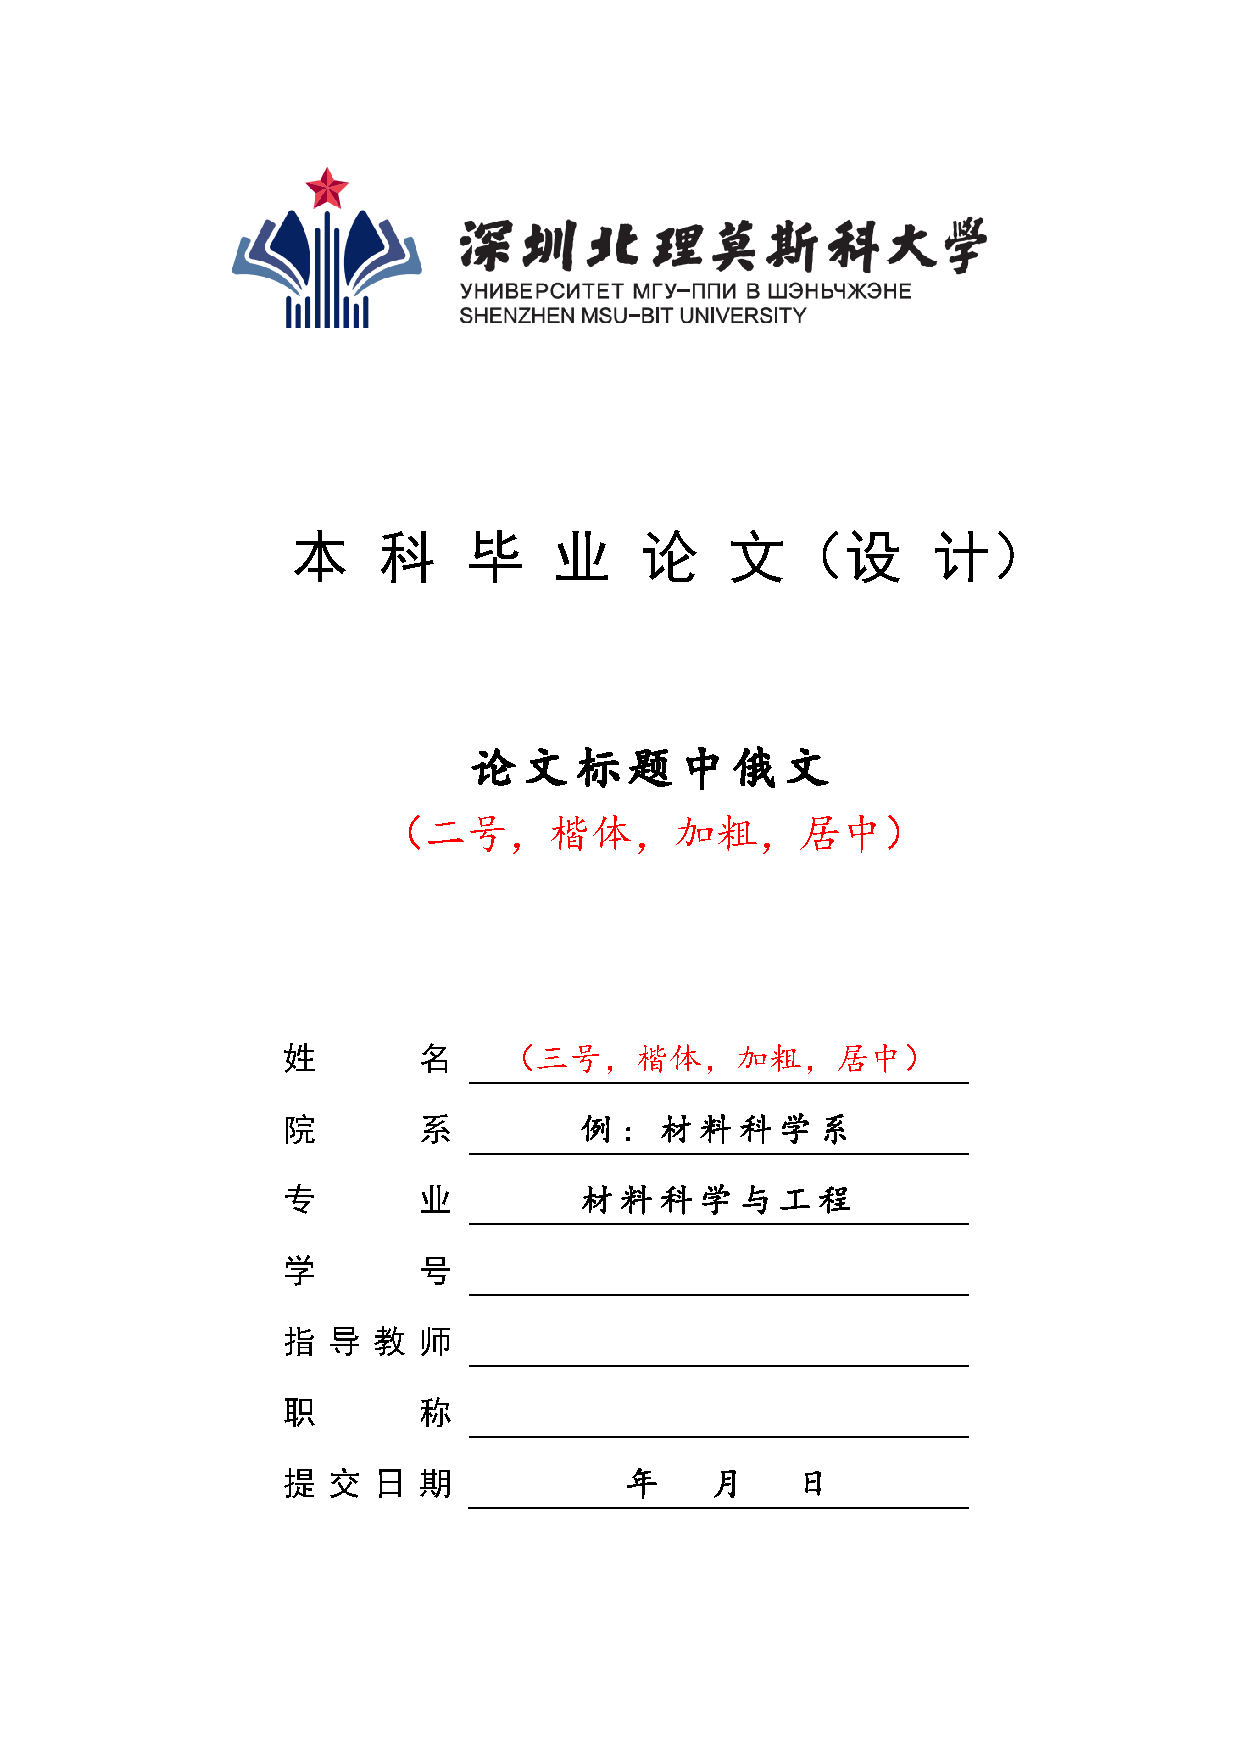
\includepdf[pages=1-4, pagecommand={\thispagestyle{fancy}}]{cover.pdf}

%---------------------------------------------------------------
% 1. 目录（中文 + 俄文）
%---------------------------------------------------------------
\cleardoublepage
\phantomsection
\printchinesetoc

\cleardoublepage
\phantomsection
\printrussiantoc

%---------------------------------------------------------------
% 2. 中文摘要
%---------------------------------------------------------------
\begin{abstractZH}
\setlength{\parindent}{2em}

轮腿机器人（wheel-legged robot）将轮式底盘的高效平动与腿式机构的可变姿态相结合，能够在结构化与半结构化环境中兼顾移动效率和地形适应性。其中，以平面五连杆并联机构作为腿、足端装驱动轮的「五连杆轮腿」构型，因结构紧凑、自由度低、力学传递清晰，被广泛用于教学与研究平台。然而，这类机器人本质上是带可变结构的车身倒立摆系统：腿长 $L_0$ 的变化会改变质心高度与转动惯量，使车身--轮子耦合系统呈现强非线性、时变特性，单一固定增益的反馈控制器难以兼顾大范围腿长变化下的平衡稳定性与运动跟踪精度，给控制器设计与算法对比研究带来了明显挑战。

针对上述问题，本文以一台名为 GBC486 的五连杆轮腿机器人为对象，构建了一条覆盖「机构建模 $\to$ MuJoCo 仿真 $\to$ 多算法控制」的完整研究方案。具体而言，本文：（1）基于平面五连杆几何关系，建立了由两个驱动关节角 $(\varphi_1, \varphi_4)$ 到虚拟腿参数 $(L_0, \varphi_0)$ 的正/逆运动学映射，并通过雅可比矩阵实现关节力矩与虚拟腿端力 $(F_0, T_p)$ 的双向变换，构成虚拟模型控制（Virtual Model Control, VMC）模块；（2）在 VMC 之上，将整车抽象为以驱动轮为底、车身为倒立摆、虚拟腿为可变长摆杆的六自由度刚体系统，状态向量取为 $\mathbf{x} = (\theta, \dot\theta, x, \dot x, \varphi, \dot\varphi)^T$，控制输入取为 $\mathbf{u} = (T, T_p)^T$，分别表示驱动轮力矩与髋部虚拟力矩；（3）基于 MuJoCo 物理引擎和原版 MJCF 模型搭建了仿真平台，采用 1\,ms 传感、4\,ms 控制、20\,ms 监控的三档周期；（4）在统一接口之上分别实现级联 PID、按腿长 $L_0$ 插值的时变 LQR 与带输入盒约束的 condensed-form MPC 三类控制器，其中 MPC 求解器采用自实现的投影梯度下降算法，无需依赖 OSQP 等外部求解器。

本文工作的主要创新点体现在三个方面：其一，提出「VMC 解耦 + 倒立摆控制 + yaw 差分 + 腿长 PID」的四通道分层控制结构，使三类控制器在同一组六维状态接口上即插即用，从机制上保障了对比的公平性；其二，将 LQR 增益矩阵 $K$ 与 MPC 模型 $(A_d, B_d, P)$ 同时按腿长 $L_0$ 离线打表、运行时线性插值，使控制律自然适应腿长变化引起的模型时变性；其三，针对 condensed QP 形式实现了带 warm-start 的投影梯度下降（PGD）求解器，单步迭代 30 次内即可收敛，避免引入外部 QP 依赖，更利于嵌入式部署。

仿真实验在平衡保持、位置阶跃、速度跟踪、yaw 阶跃、腿长动态变化以及瞬态扰动恢复六类工况下完成。结果表明：在腿长 $L_0 \in [0.10, 0.40]\,\mathrm{m}$ 范围内，PID 控制器在 $L_0 \approx 0.20\,\mathrm{m}$ 标定点附近表现稳定但腿长偏离时易出现持续振荡；LQR 借助按 $L_0$ 插值的增益表保持了全程稳定；MPC 在轮力矩饱和（$|T| \le 4\,\mathrm{N\cdot m}$）的扰动恢复工况中通过显式约束维持了输入合法性，姿态误差峰值显著低于 PID。

本研究为五连杆轮腿机器人控制系统的设计与算法选型提供了量化的仿真依据，并可作为后续轮腿一体化运动规划、地形自适应平衡以及基于学习的控制研究的统一基础平台。

\keywordsZH{轮腿机器人；五连杆并联机构；虚拟模型控制；MuJoCo；线性二次型调节器；模型预测控制}
\end{abstractZH}

%---------------------------------------------------------------
% 3. 俄文摘要（占位，可后续补充翻译）
%---------------------------------------------------------------
\begin{abstractRU}
\setlength{\parindent}{2em}

% TODO: 俄文摘要待翻译补充。

\keywordsRU{колёсно-шагающий робот; пятизвенный параллельный механизм; виртуальная модельная регулировка; MuJoCo; линейно-квадратичный регулятор; модельно-предиктивная регулировка}
\end{abstractRU}

%---------------------------------------------------------------
% 4. 英文摘要
%---------------------------------------------------------------
\begin{abstractEN}
\setlength{\parindent}{2em}

Wheel-legged robots combine the locomotion efficiency of wheels with the posture flexibility of legs, making them attractive for both structured and semi-structured environments. Among them, a planar five-bar linkage leg with a wheel mounted at the end-effector---referred to as a five-bar wheel-legged structure---is widely used in teaching and research platforms thanks to its compactness, low degree-of-freedom count, and clear force-transmission path. Such a robot, however, is fundamentally a wheeled inverted pendulum with a variable-structure leg: changes in leg length $L_0$ alter both the center-of-mass height and the moment of inertia, giving the body--wheel coupled system strong nonlinearity and time-varying dynamics, so that controllers with fixed gains struggle to maintain both balance and motion tracking across a wide range of leg lengths.

This thesis targets a five-bar wheel-legged robot named GBC486 and develops a complete research pipeline covering mechanical modeling, MuJoCo-based simulation, and multi-algorithm control. Specifically, this work: (1) builds the forward and inverse kinematics from the two driven joint angles $(\varphi_1, \varphi_4)$ to the virtual leg parameters $(L_0, \varphi_0)$ based on planar five-bar geometry, and uses the Jacobian to map between joint torques and the virtual leg-end force/torque $(F_0, T_p)$, forming the Virtual Model Control (VMC) module; (2) on top of VMC, abstracts the robot as a wheeled inverted pendulum with a variable-length swing rod, takes the state vector as $\mathbf{x} = (\theta, \dot\theta, x, \dot x, \varphi, \dot\varphi)^T$ and the control input as $\mathbf{u} = (T, T_p)^T$, where $T$ is the wheel torque and $T_p$ the virtual hip torque; (3) builds a simulation platform on MuJoCo using the original MJCF model with a three-tier loop (1\,ms sensing / 4\,ms control / 20\,ms monitoring); (4) implements three balance controllers behind a unified interface---a cascaded PID, an LQR whose feedback gain $K$ is interpolated online over $L_0$, and a condensed-form linear MPC with input box constraints---where the MPC solver is implemented in-house via projected-gradient descent (PGD), without depending on external QP solvers such as OSQP.

Three contributions are highlighted. First, a four-channel hierarchical control architecture---``VMC decoupling + inverted-pendulum control + yaw differential + leg-length PID''---is proposed so that the three controllers can be plugged into the same six-dimensional state interface, structurally guaranteeing fair comparison. Second, both the LQR gain $K$ and the MPC model triplet $(A_d, B_d, P)$ are tabulated offline against $L_0$ and linearly interpolated online, naturally accommodating the time variation introduced by changing leg length. Third, a warm-started PGD solver is implemented in condensed QP form, converging within 30 iterations per step, avoiding external solver dependencies and easing embedded deployment.

Simulation experiments are conducted under six scenarios: balance keeping, position step, velocity tracking, yaw step, leg-length dynamic change, and transient disturbance recovery. Within $L_0 \in [0.10, 0.40]\,\mathrm{m}$, PID is stable around the calibration point ($L_0 \approx 0.20\,\mathrm{m}$) but tends to oscillate when the leg length deviates; LQR remains stable across the whole range thanks to the $L_0$-indexed gain table; MPC, when the wheel torque saturates ($|T| \le 4\,\mathrm{N\cdot m}$) during disturbance recovery, preserves input feasibility through the explicit constraint and yields markedly lower peak posture error than PID.

This work provides a quantitative simulation basis for the design and algorithm selection of five-bar wheel-legged robot control systems, and can serve as a foundation for subsequent research on integrated wheel-leg motion planning, terrain-adaptive balance, and learning-based control.

\keywordsEN{Wheel-legged robot; Five-bar parallel mechanism; Virtual Model Control; MuJoCo; Linear quadratic regulator; Model predictive control}
\end{abstractEN}

\ctexset{chapter/afterskip=0.5ex}
\printtitle
\ctexset{chapter/break={}, chapter/beforeskip=0.5ex}

%===============================================================
% 第一章 前言
%===============================================================
\chapter{前言}
\russianchaptertitle{Введение}
\ctexset{chapter/break=\clearpage, chapter/beforeskip=1ex, chapter/afterskip=2ex}

\section{研究背景和意义}
\russiansectiontitle{Актуальность темы исследования}

近十年来，移动机器人在工业巡检、室内服务、教育科研等场景中扮演的角色日益重要。在众多构型中，纯轮式机器人虽然平动效率高、控制简单，但跨越障碍能力受限；纯腿式机器人地形适应能力强，却伴随高复杂度的步态规划与较低的运动效率。\textbf{轮腿机器人（wheel-legged robot）}通过把驱动轮安装在腿式机构末端，将两者优势结合：在平地上以轮式高速通行，在台阶或斜坡上则借腿部姿态调整改变车身高度与重心，从而在不显著增加运动学维度的前提下扩展工作空间\cite{Bjelonic2019KeepRollin,Klemm2019Ascento,Wang2021WheelLegged}。从波士顿动力 Handle、ETH Zurich 的 Ascento，到国内多款教学/竞赛平台，轮腿机器人正成为兼具研究价值与工程价值的代表性对象。

在轮腿机器人中，以\textbf{平面五连杆并联机构}作为腿部、足端安装驱动轮的「五连杆轮腿」构型尤具代表性。其每条腿仅由两个驱动关节驱动，但通过五连杆几何约束生成可变腿长 $L_0$ 与虚拟腿极角 $\varphi_0$，自由度低、传动链紧凑、维护成本可控，非常适合作为本科教学与算法验证平台\cite{Yoneda1994SkyHook,Tsai1999RobotAnalysis}。然而，这种「机体 + 双五连杆腿 + 双轮」的构型在控制层面上等价于一个\textbf{车身倒立摆系统}：当 $L_0$ 变化时，车身质心高度、等效摆杆长度以及绕髋轴的转动惯量都会同步改变，导致从轮力矩 $T$ 与髋部虚拟力矩 $T_p$ 到状态量的传递特性随 $L_0$ 时变\cite{Pathak2005WheeledIP}。这一时变特性使得固定增益控制律在大腿长变化范围下容易出现稳态偏移、振荡甚至失稳，因此围绕该构型开展系统化的运动建模、仿真验证与控制算法对比研究，具有较强的工程意义。

进一步地，五连杆轮腿机器人的控制问题天然涵盖了多个层级的控制对象：底层是关节力矩--腿长/腿角的并联机构传递（适合用虚拟模型控制 VMC 解耦）；中层是车身倒立摆的姿态--平动耦合（适合用经典反馈控制、最优控制或预测控制）；高层是 yaw 跟踪与腿长跟踪等任务级控制。已有相关工作多侧重单一层级的算法改进（例如仅关注倒立摆 LQR 控制\cite{AndersonMoore1990OptControl,KwakernaakSivan1972LinearOpt}，或仅关注 MPC 在轮式机器人上的应用\cite{Mayne2000ConstrainedMPC}），鲜有研究在统一对象、统一仿真平台与统一接口上对 PID、LQR、MPC 三类典型控制范式开展端到端的对比，并系统地处理由 $L_0$ 引起的时变特性。这一空白给轮腿机器人控制器选型与教学示范带来了明显的工程门槛。

针对上述问题，本课题以 GBC486 五连杆轮腿机器人为研究对象，构建了一条「机构建模 $\to$ 仿真验证 $\to$ 多算法控制」的完整研究方案。课题在控制层引入了「VMC 解耦 + 倒立摆控制 + yaw 差分 + 腿长 PID」的四通道分层结构，并将 LQR 增益与 MPC 预测模型按 $L_0$ 离线打表、运行时线性插值，从而使同一组接口可以无缝承载三种典型控制范式。所形成的统一仿真平台与对比实验框架，一方面可为五连杆轮腿机器人控制器的设计与调参提供量化依据，另一方面也可作为后续地形自适应平衡、跳跃越障以及基于学习的控制研究的基础平台，具有较强的延展性和教学示范价值。

\section{研究目标与论文结构}
\russiansectiontitle{Цели исследования и структура работы}

本课题的总体研究目标是：以 GBC486 五连杆轮腿机器人为对象，建立一套从机构建模到仿真验证的完整研究方案，并在统一的仿真平台与统一的状态接口下完成 PID、LQR 与 MPC 三类典型控制方法的实现与系统化对比，为轮腿机器人控制系统的设计与算法选型提供量化的仿真依据。

为实现上述总目标，本研究将其拆分为以下四个相互衔接的子目标：

\begin{enumerate}
\item \textbf{建模目标}：建立五连杆并联机构的正/逆运动学映射与雅可比矩阵，以及车身--轮子耦合系统的六维倒立摆动力学方程，明确状态向量、控制输入及其与底层关节量的换算关系，为仿真模型搭建与控制器设计提供统一的数学基础；
\item \textbf{仿真平台目标}：基于 MuJoCo 物理引擎与原版 MJCF 模型，构建包含传感器、执行器和外部指令接口的仿真平台，确保三类控制器能够在同一环境、同一参数和同一工况下进行测试与对比，提升实验结果的可比性和可复现性；
\item \textbf{控制算法目标}：分别实现级联 PID、按腿长 $L_0$ 插值的时变 LQR、以及 condensed QP 形式带输入盒约束的 MPC 三类控制器，覆盖经典反馈控制、最优控制和预测控制三种典型范式，并在覆盖平衡保持、位置/速度跟踪与扰动恢复的多种工况下完成参数整定与性能评估；
\item \textbf{对比分析目标}：在统一仿真平台上对三类控制器进行横向对比，分析 $L_0$ 变化、扰动大小与控制约束对响应特性的影响，量化各方法的适用边界与工程取舍。
\end{enumerate}

\textbf{本论文的主要结构安排如下}：第一章为前言，介绍课题的研究背景、意义、研究目标及论文结构；第二章为相关研究，系统综述轮腿机器人建模方法、五连杆并联机构与虚拟模型控制、车身倒立摆控制以及 PID、LQR、MPC 三类控制算法的研究现状，并将其与本研究方案相挂钩；第三章为系统设计与框架，给出本系统的总体架构以及建模、仿真平台、控制算法和外部交互四个模块的设计思路；第四章为系统实现与实验结果，详细描述各模块的具体实现方式、关键公式与参数选取，并通过六类典型工况下的仿真实验对三类控制算法进行量化对比分析；第五章为总结与展望，回顾本文主要工作与创新点，分析当前方案的不足，并对未来可拓展的研究方向（包括实物部署）进行展望。

%===============================================================
% 第二章 相关研究
%===============================================================
\chapter{相关研究}
\russianchaptertitle{Обзор литературы}

五连杆轮腿机器人的运动仿真与控制研究涉及轮腿机器人构型、五连杆并联机构与虚拟模型控制、车身倒立摆动力学建模、物理仿真平台以及 PID/LQR/MPC 三类典型控制算法等多个方面。本章按照「机构 $\to$ 平台 $\to$ 控制算法」的脉络，对国内外相关研究进行综述，并在每一小节末尾说明本研究在该方向上的方法选择，以便后续章节中的具体设计与实现有据可循。

\section{轮腿机器人构型与建模}
\russiansectiontitle{Конфигурация и моделирование колёсно-шагающих роботов}

轮腿机器人本质上是兼具腿式机构姿态自由度与轮式驱动效率的混合移动平台。Bjelonic 等人\cite{Bjelonic2019KeepRollin}系统综述了近年来轮腿机器人研究进展，指出轮腿构型按「轮在足端 / 轮独立挂在腿侧」等不同布局可分为多类，其中「轮在足端」的构型由于腿部直接承载整车重量并通过轮子提供平动驱动，控制问题最贴近车身倒立摆模型。Klemm 等人提出的 Ascento\cite{Klemm2019Ascento}是这一构型的代表性工作之一：双连杆并联腿 + 末端驱动轮，配合躯干姿态控制可实现自平衡、阶梯越障与跳跃。我国近年来也涌现出 Diablo、Ollie 等基于双轮腿的研究/教学平台\cite{Wang2021WheelLegged}，为算法验证与对比提供了实验基础。

在建模方面，研究者通常将整车抽象为以驱动轮为底、车身为倒立摆的多体系统。Pathak 等人针对带驱动轮的倒立摆给出了经典动力学方程与稳定性分析\cite{Pathak2005WheeledIP}，明确指出当摆杆长度（对应轮腿机器人中的腿长 $L_0$）变化时，整个系统呈现典型的时变线性化特性。Fang\cite{Fang2014PSOLQR}在双轮自平衡机器人上以拉格朗日法建立动力学模型，并通过粒子群优化算法整定 LQR 权重矩阵，从模型与权重整定两个角度展示了精细化建模对平衡控制性能的影响。这些工作共同表明：将轮腿机器人在小角度近似下视为带变长摆杆的倒立摆，是控制器设计阶段可被广泛接受的合理简化。

考虑到本研究面向的 GBC486 机器人为典型的「机体 + 双五连杆腿 + 双轮」构型，且关注的核心控制问题包括平衡保持、位置/速度跟踪与扰动恢复，本研究在第~\ref{ch:impl}~章中将以「五连杆并联机构 + 车身倒立摆」作为统一建模基础，将整车状态归约为六维状态向量 $(\theta, \dot\theta, x, \dot x, \varphi, \dot\varphi)$，并保留腿长 $L_0$ 作为模型参数，以便后续 LQR、MPC 控制器对 $L_0$ 进行参数化。

\section{五连杆并联机构与虚拟模型控制}
\russiansectiontitle{Пятизвенный параллельный механизм и виртуальная модельная регулировка}

平面五连杆并联机构（A-B-C-D-E 五铰）由两个驱动关节通过两组三连杆并联约束驱动末端工作点，是足式机器人腿部机构的经典构型之一。Tsai 在其并联机构经典专著\cite{Tsai1999RobotAnalysis}中系统给出了串/并联机构的位置分析、雅可比、刚度与动力学分析框架，为五连杆腿的运动学建模与雅可比推导提供了基础参考；Yoneda 等人\cite{Yoneda1994SkyHook}在四足机器人姿态控制中提出了 sky-hook 悬挂控制思想，对腿式机构的多自由度力学耦合分析具有借鉴价值。

针对五连杆腿的控制，直接在关节空间设计反馈律会受到雅可比方向耦合的影响，调参困难。Pratt 等人提出的\textbf{虚拟模型控制（Virtual Model Control, VMC）}\cite{Pratt2001VMC}通过把腿端等效为可控的虚拟弹簧/连杆，将期望的虚拟腿端力或力矩通过雅可比转置映射回关节力矩，从而把高维关节空间的控制问题降维为低维虚拟空间的力/力矩控制，已被广泛应用于双足、四足及轮腿机器人腿部子系统中。在五连杆构型上，VMC 自然将关节空间的两个驱动量映射为两个虚拟量：等效腿长方向支撑力 $F_0$ 与髋部虚拟力矩 $T_p$。其中 $F_0$ 用于控制腿长 $L_0$，$T_p$ 用于控制车身倾角，从而把腿部的「姿态」与「长度」两个任务分通道处理。

综合考虑工程实现的清晰度与多算法对比的便捷性，本研究在第~\ref{ch:impl}~章中将沿用 Pratt 等人的 VMC 框架：基于五连杆几何关系导出 $(\varphi_1, \varphi_4) \to (L_0, \varphi_0)$ 的正运动学与雅可比矩阵，再将上层平衡控制器输出的 $(F_0, T_p)$ 通过雅可比映射回关节力矩 $(\tau_1, \tau_4)$，作为关节执行器的最终控制量。

\section{车身倒立摆控制方法概述}
\russiansectiontitle{Обзор методов управления телом-маятником}

车身倒立摆是研究轮腿机器人平衡控制的基础对象。围绕这一对象的控制方法可大致分为三类：以 PID 为代表的经典反馈控制、以 LQR/LQI 为代表的最优控制，以及以 MPC 为代表的预测控制\cite{Pathak2005WheeledIP,AndersonMoore1990OptControl,KwakernaakSivan1972LinearOpt}。其中 PID 控制结构简单、调参经验丰富，但在系统呈现时变或多通道耦合特性时调试代价显著上升\cite{Astrom1995PID}；LQR 通过状态空间模型与二次型代价函数取得稳定性与控制能耗的最优折中，在小角度近似下与倒立摆模型天然契合\cite{AndersonMoore1990OptControl}；MPC 则通过滚动优化在每一步显式处理状态、输入及其增量约束，特别适合带饱和或安全约束的系统\cite{Mayne2000ConstrainedMPC,Rawlings2017MPC}。

在轮腿机器人这一具体对象上，研究者已经开展了若干代表性工作。Klemm 等人在 Ascento 上采用 LQR 完成了双轮自平衡控制\cite{Klemm2019Ascento}，并进一步在带运动学闭环的轮式双足机器人上提出了 LQR 辅助的全身控制框架\cite{Klemm2020LQRWBC}，将 LQR 作为一项运动任务嵌入分层控制中以处理非最小相位平衡动力学；Fang\cite{Fang2014PSOLQR}通过粒子群算法对两轮自平衡机器人的 LQR 权重矩阵 $Q$, $R$ 做了系统化整定，展示了权重整定对响应特性的显著影响；Bouzoualegh 等人则在轮式机器人上展示了 MPC 通过显式约束处理轮力矩饱和的优势\cite{Bouzoualegh2018DiffDriveMPC}。这些工作共同支持了「基于线性化模型的状态反馈/预测控制是轮腿平衡问题的合理选择」这一判断。

考虑到本研究的对比目标是以同一对象、同一接口横向评估 PID、LQR、MPC 三类控制范式，本课题在第~\ref{ch:impl}~章中将分别实现：（1）作为工程基线的级联 PID，包含关节位置内环、pitch 平衡内环、位移外环以及 yaw 差分共四级；（2）按腿长 $L_0$ 离线打表的时变 LQR；（3）在 LQR 模型基础上引入预测时域与输入约束的 MPC。三类控制器共享相同的六维状态向量与二维控制输入。

\section{LQR 增益调度与时变线性化}
\russiansectiontitle{Планирование коэффициентов усиления LQR и линеаризация на временно-зависимых интервалах}

经典 LQR 的最优反馈律建立在线性时不变（LTI）系统假设之上，其反馈增益 $K$ 由代数 Riccati 方程一次性求出\cite{AndersonMoore1990OptControl,KwakernaakSivan1972LinearOpt}。然而在轮腿机器人中，$L_0$ 的变化会显著改变车身质心高度、等效摆杆长度与转动惯量，使从控制输入到状态导数的雅可比矩阵随 $L_0$ 时变。直接采用单一工作点的 LQR 增益会在 $L_0$ 偏离标定点时退化甚至失稳\cite{Wang2021WheelLegged,Klemm2020LQRWBC}。

针对这一问题，已有研究主要采用两类策略：一是\textbf{LQR 增益调度（gain scheduling）}\cite{RughShamma2000GainSched}，对若干典型工作点离线求解 LQR 并在运行时根据实测变量插值；二是基于轨迹线性化的\textbf{迭代 LQR（iLQR）}\cite{Tassa2012iLQR}，逐步沿轨迹更新增益。前者实现简单、运行时开销极低，特别适合像 $L_0$ 这样变化范围有限的参数；后者精度更高但需要在线求解 Riccati，对嵌入式平台不够友好。

考虑到本研究在仿真平台上需要对算法机制本身进行可控的对比，本课题在第~\ref{ch:impl}~章中采用增益调度策略：在 $L_0 \in [0.10, 0.40]\,\mathrm{m}$ 范围内取 30 个等距样点，离线求解每点的连续 ARE，得到对应的 $K$ 矩阵查找表，运行时按当前 $L_0$ 做线性插值。这一策略既保留了 LQR 的解析最优性，又能自然适应腿长变化引起的模型时变性。

\section{模型预测控制与求解器选型}
\russiansectiontitle{Модельно-предиктивная регулировка и выбор решателя}

模型预测控制（Model Predictive Control, MPC）在每个控制周期内求解一个有限时域内的优化问题，得到最优控制序列后仅执行第一步控制输入，并在下一个周期重新求解\cite{Mayne2000ConstrainedMPC,Maciejowski2002Predictive}。MPC 的核心优势在于能显式纳入状态、输入及其增量约束，因此在涉及饱和或安全边界的系统中具有天然优势。在轮腿机器人这类带轮力矩饱和的系统中，MPC 能够在扰动恢复或剧烈机动期间通过约束保持输入合法性。

针对线性 MPC 的实时求解，研究者通常将其转化为标准二次规划（QP）问题。常见的实现方案包括：基于 OSQP\cite{Stellato2020OSQP}、qpOASES 等通用 QP 求解器的工程实现；基于 condensed-form（消去状态变量、仅保留控制序列为决策变量）的紧凑实现\cite{Rawlings2017MPC,Maciejowski2002Predictive}；以及面向嵌入式部署的\textbf{投影梯度下降（PGD）}等一阶方法\cite{Patrinos2014AcceleratedDGP}。其中 condensed form + PGD 由于不依赖外部库、内存占用低、迭代结构简单，特别适合嵌入式 MCU 与教学示范场景。

考虑到本研究面向教学与算法对比、且希望避免引入额外的外部依赖，本课题在第~\ref{ch:impl}~章中采用 condensed form + warm-start PGD 的求解策略：每步通过将上一周期解整体左移一位作为本周期 warm start，PGD 迭代 30 次内即可收敛到与外部 QP 求解器接近的解。终端代价矩阵 $P$ 由 LQR 用的离散 Riccati 方程一次性求得。

\section{仿真平台}
\russiansectiontitle{Платформа симуляции}

仿真平台是机器人控制研究的关键支撑工具，其作用包括隔离硬件不确定性、缩短算法迭代周期、提供统一的对比测试基础。当前主流的机器人仿真平台主要包括 Gazebo、Webots 与 MuJoCo 等。Gazebo 与 ROS 深度集成，适合系统级仿真，但物理求解步长较大；Webots 在教育场景中应用广泛，但场景复杂度提升时求解效率会有所下降。

MuJoCo（Multi-Joint dynamics with Contact）由 Todorov 等人提出\cite{Todorov2012MuJoCo}，是专为基于模型的控制研究设计的物理仿真引擎。其在接触建模、关节求解和数值稳定性方面进行了专门优化，支持小步长高频仿真，并提供了简洁的 MJCF（MuJoCo XML）模型描述格式与多语言绑定接口（C/C++、Python 等）。在轮腿机器人这类多刚体接触系统中，MuJoCo 既能稳定地仿真轮地接触与并联机构内力，又能以较高的实时倍率运行，因此被广泛用于双足、四足及轮腿机器人控制算法研究\cite{Hwangbo2019Agile,Hutter2017ANYmal}。基于上述特性，本研究选择 MuJoCo 作为五连杆轮腿机器人仿真平台的核心引擎，并在第~\ref{ch:design}~章中给出基于 MJCF 的机器人模型与统一控制接口设计。

\section{本章小结}
\russiansectiontitle{Выводы}

本章围绕五连杆轮腿机器人的运动仿真与控制研究，从机构构型、五连杆并联机构与虚拟模型控制、车身倒立摆控制、LQR 增益调度、MPC 求解器选型以及仿真平台六个方面对国内外相关工作进行了梳理。在机构方面，本研究将沿用「机体 + 双五连杆腿 + 双轮」的典型构型并在控制层抽象为车身倒立摆模型；在控制方面，分别采用级联 PID、按 $L_0$ 增益调度的 LQR 与 condensed-form + PGD 求解的 MPC 三类典型方法；在平台方面选择 MuJoCo 作为统一仿真引擎。基于以上综述，本研究将在第~\ref{ch:design}~章中给出涵盖建模、仿真平台、控制算法和外部交互的系统总体设计。

%===============================================================
% 第三章 系统设计与框架
%===============================================================
\chapter{系统设计与框架}\label{ch:design}
\russianchaptertitle{Проектирование системы}

本章在第~2~章相关研究的基础上，围绕「机构建模 $\to$ 仿真验证 $\to$ 多算法控制」的总体研究目标，给出本课题的系统总体架构和各模块的设计思路。本章只关注模块的功能定位、组成结构以及设计理由（即「做什么」与「为什么」），具体的数学推导、参数设定与代码实现细节在第~\ref{ch:impl}~章中给出。

\section{总体架构概述}
\russiansectiontitle{Общая архитектура системы}

为了在统一的实验环境下完成 PID、LQR 与 MPC 三类典型控制方法在五连杆轮腿机器人上的对比，本研究将整体系统划分为四个相互衔接的模块：\textbf{机构与动力学建模模块}、\textbf{MuJoCo 仿真平台模块}、\textbf{控制算法模块}和\textbf{外部交互与监控模块}。其中，建模模块负责给出五连杆运动学/雅可比与车身倒立摆动力学的统一描述；仿真平台模块基于 MJCF 在 MuJoCo 内构建物理实体并按「传感 1\,ms / 控制 4\,ms / 监控 20\,ms」的三档周期运行；控制算法模块在仿真平台提供的统一接口之上，实现 PID、LQR、MPC 三类控制器；外部交互与监控模块负责通过 UDP 指令服务器接收用户输入的目标值（速度、yaw、腿长等）并将运行状态导出供分析。

\begin{figure}[H]
  \centering
  
\includegraphics[width=0.95\textwidth]{fig1_system_framework}
  \caption{系统总体框架图}
  \label{fig:framework}
\end{figure}

如\cref{fig:framework}所示，整套系统以「统一接口 + 控制律可替换」为核心：建模模块同时向仿真平台和控制算法提供机构参数、雅可比与线性化模型；仿真平台向控制器输出六维状态 $\mathbf{x}$ 与底层关节量，并接收控制器返回的关节力矩与轮力矩，构成闭环；控制算法模块对外提供统一的 \texttt{compute(imu, motors)} $\to$ \texttt{(joint\_torque, wheel\_torque)} 接口，使三种控制器可以在不修改仿真环境的前提下相互替换；外部交互模块以 UDP 形式注入目标，使所有工况实验都可以通过同一份脚本驱动。这一架构的核心特点是\textbf{接口统一}与\textbf{控制律可替换}：所有控制器面对相同的六维状态与二维控制输入，避免因接口差异引入额外的对比偏差。

\section{机构与动力学建模模块设计}
\russiansectiontitle{Модуль моделирования механизма и динамики}

机构与动力学建模模块是整个系统的数学基础，其功能定位是：以统一的状态变量、控制输入和动力学描述，为仿真平台搭建与控制器设计提供共同的数学模型。该模块包含三个子组件：\textbf{五连杆运动学与雅可比}、\textbf{虚拟模型控制（VMC）映射}和\textbf{车身倒立摆动力学}。五连杆运动学子组件负责将两个驱动关节角 $(\varphi_1, \varphi_4)$ 映射为虚拟腿长 $L_0$ 与虚拟腿极角 $\varphi_0$，并提供对应的雅可比矩阵；VMC 映射子组件利用雅可比将上层期望的虚拟腿端力 $F_0$（控制腿长）与髋部虚拟力矩 $T_p$（控制车身倾角）变换为关节力矩 $(\tau_1, \tau_4)$；车身倒立摆动力学子组件则在 VMC 之上，将整车抽象为以驱动轮为底、车身为倒立摆、虚拟腿为可变长摆杆的六自由度刚体系统，建立从控制输入到状态导数的非线性微分方程。

\begin{figure}[H]
  \centering
  
\includegraphics[width=0.95\textwidth]{fig2_robot_structure}
  \caption{GBC486 机器人结构示意图}
  \label{fig:robot}
\end{figure}

\begin{figure}[H]
  \centering
  
\includegraphics[width=0.95\textwidth]{fig3_five_bar_kinematics}
  \caption{五连杆机构与虚拟腿参数定义}
  \label{fig:fivebar}
\end{figure}

\cref{fig:fivebar} 给出了单条腿五连杆机构与虚拟腿之间的参数对应关系：固定铰 $A$、$E$ 安装于机体，中点 $M = (l_5/2, 0)$ 取为虚拟腿极点；驱动关节角 $(\varphi_1, \varphi_4)$ 经闭链约束解出从动角 $(\varphi_2, \varphi_3)$，进而由几何关系得到虚拟腿长 $L_0 = |MC|$ 与极角 $\varphi_0$。上层平衡控制器输出的虚拟腿端力 $F_0$（沿 $MC$ 方向）与髋部虚拟力矩 $T_p$ 经雅可比 $J(\varphi_1, \varphi_4)$ 反映射为驱动关节力矩 $(\tau_1, \tau_4)$，由此把多杆耦合的关节空间控制问题降维为「腿长 + 车身倾角」两个解耦通道。

设计上之所以采用「五连杆 VMC + 倒立摆」的双层建模思路，是因为五连杆机构在关节空间下耦合严重、调参困难，而 VMC 将其降维为两个物理直观的虚拟控制量，从而把「腿长跟踪」与「车身平衡」两个任务自然分通道处理。在 VMC 之上再以倒立摆模型描述车身平衡问题，状态向量 $\mathbf{x} = (\theta, \dot\theta, x, \dot x, \varphi, \dot\varphi)^T$ 中前两项描述虚拟腿摆角，中两项描述车身平动，后两项描述车身倾角，构成完整的小角度倒立摆模型。模块对外仅暴露「VMC 正/逆运动学、雅可比、连续/离散动力学函数」三组接口，对内屏蔽具体推导细节。

\section{仿真平台模块设计}
\russiansectiontitle{Модуль платформы симуляции}

仿真平台模块的核心功能定位是：基于 MuJoCo 物理引擎与原版 MJCF 模型，构建一个\textbf{可重复、可观测、易扩展}的五连杆轮腿机器人测试环境，为三类控制器提供统一的测试基础。该模块包括\textbf{机器人 MJCF 模型}、\textbf{传感器接口}、\textbf{执行器接口}以及\textbf{多档周期主循环}四个子组件。MJCF 模型按照「机体（base）+ 双腿四关节（jAB/jAG, jIJ/jIO）+ 双驱动轮（jwheel\_right/jwheel\_left）」的层级结构组织，所有连杆几何均由原始 STL 网格描述；传感器接口暴露 IMU（欧拉角 + 角速度）、四个关节编码器和两个轮编码器；执行器接口提供四个关节力矩通道与两个轮力矩通道，并通过 \texttt{gainprm} 处理左轮的方向反转；多档周期主循环则将物理仿真步进、传感器读取、控制计算与监控输出按 1\,ms / 1\,ms / 4\,ms / 20\,ms 的整数倍关系协同推进，确保物理求解稳定性的同时支持上层控制频率的工程合理性。

\begin{figure}[H]
  \centering
  \figplaceholder[0.32]{图 4 仿真平台架构图 ——「模型层 / 物理仿真层 / 接口层 / 主循环层」四层结构与多档周期协同}
  \caption{仿真平台架构图}
  \label{fig:simplatform}
\end{figure}

如\cref{fig:simplatform}所示，仿真平台模块按「模型层 $\to$ 物理仿真层 $\to$ 接口层 $\to$ 主循环层」的纵向结构组织：模型层完成 MJCF 文件加载与参数注入；物理仿真层由 MuJoCo 内核负责积分求解；接口层将 IMU/编码器读数和执行器写入封装为 Python 端的状态读取/控制写入函数；主循环层则按多档周期编排各子任务。该模块的设计重点有三：其一，仿真步长与控制周期严格分离，以保证物理求解稳定性的同时支持不同频率的上层控制；其二，所有传感器与控制接口均以「IMU + 关节电机数据 + 轮电机数据」的统一形式对外暴露，与建模模块中的接口约定保持一致；其三，机器人模型直接复用原版 MJCF 文件，避免简化几何带来与实物的差异。

\section{控制算法模块设计}
\russiansectiontitle{Модуль алгоритма управления}

控制算法模块是本研究的核心，其功能定位是为五连杆轮腿机器人提供 PID、LQR 与 MPC 三类典型平衡控制策略，并通过统一的输入--输出接口接入仿真平台。所有控制器共享同一组六维状态量 $(\theta, \dot\theta, x, \dot x, \varphi, \dot\varphi)$ 和同一组二维平衡控制量 $(T, T_p)$，并对外提供形式一致的 \texttt{compute(imu, motors)} $\to$ \texttt{(joint\_torque, wheel\_torque)} 接口。所有控制器内部都包含一致的辅助通道：\textbf{腿长 PID + 重力前馈}生成 $F_0$ 用于控制腿长，\textbf{yaw PID} 在轮力矩上叠加差分用于跟踪 yaw，\textbf{VMC 雅可比}将 $(F_0, T_p)$ 变换为关节力矩。差异仅集中在如何生成核心平衡量 $(T, T_p)$ 上。

\begin{figure}[H]
  \centering
  \figplaceholder[0.30]{图 5 三类控制器统一接口框图 —— PID / LQR / MPC 共享同一 \texttt{compute(imu, motors)} 接口，差异仅集中在平衡量 $(T, T_p)$ 的生成}
  \caption{三类控制器统一接口框图}
  \label{fig:ctrlif}
\end{figure}

\subsection{PID 控制器设计思路}
\russiansubsectiontitle{Концепция проектирования PID-регулятора}

PID 控制器作为对照基线，采用四级联结构：关节位置 PID（基于 VMC 逆运动学得到的关节目标）、pitch 内环（车身倾角 $\to$ 轮力矩 $T$）、位移外环（位移误差 $\to$ pitch 参考）、yaw 差分（yaw 误差 $\to$ 左右轮差分力矩）。这种结构沿用工程上常见的「内快外慢」分层调参思路，便于通过分通道独立调参实现稳定基础控制；其局限在于不能显式利用六维状态模型与系统约束信息。

\subsection{LQR 控制器设计思路}
\russiansubsectiontitle{Концепция проектирования LQR-регулятора}

LQR 控制器以车身倒立摆动力学在零工作点附近的线性化模型为基础，将整车六维状态作为反馈变量，构建标准的状态空间形式，并通过求解连续代数 Riccati 方程得到最优状态反馈律 $K$。考虑到腿长 $L_0$ 的变化会显著改变线性化模型，本研究在设计上对若干典型 $L_0$ 值离线求解 LQR，运行时根据实测 $L_0$ 做\textbf{线性插值}（gain scheduling），从而使控制律自然适应腿长变化引起的模型时变性。权重矩阵 $Q$, $R$ 被设计为对外暴露的可调超参数。

\subsection{MPC 控制器设计思路}
\russiansubsectiontitle{Концепция проектирования MPC-регулятора}

MPC 控制器在 LQR 所用线性化模型的基础上进一步引入有限预测时域与显式输入约束。每个控制周期内，MPC 求解一个 condensed form 的二次规划问题，得到未来若干步的最优控制序列，并仅执行其中第一步。设计上着重处理三类要素：（1）状态--代价以 LQR 的 Riccati 解作为终端代价 $P$，保证滚动稳定性；（2）控制量约束（轮力矩饱和、髋部虚拟力矩物理上限）以盒约束形式注入；（3）求解器层面采用自实现的投影梯度下降（PGD）+ warm start，避免引入外部 QP 依赖。MPC 控制器的设计目标不在于追求理论上的最优性，而是体现「显式建模 + 显式约束」在轮力矩饱和场景下的实际优势。

\section{外部交互与监控模块}
\russiansectiontitle{Модуль внешнего взаимодействия и мониторинга}

外部交互与监控模块的功能定位是把仿真平台与控制算法暴露给用户/上层脚本，使工况切换、目标修改与运行监控不需要改动控制器代码。模块包括 \textbf{UDP 指令服务器}、\textbf{状态打印/日志}与\textbf{键盘控制}三个子组件。UDP 指令服务器在固定端口监听速度、yaw、腿长等目标值的更新，将其热更新到控制器的目标缓存；状态打印/日志组件将状态估计器的关键变量按设定周期输出，便于在不同工况下进行响应曲线绘制；键盘控制组件则提供运行时的人工干预通道。这一模块虽不参与控制计算本身，但其存在保证了「同一份控制器代码 + 同一仿真二进制 + 多种实验工况」的实验工作流。

\begin{figure}[H]
  \centering
  \figplaceholder[0.28]{图 5' 外部交互框图 —— UDP 指令服务器 / 键盘控制 / 状态日志 三通道与控制器目标缓存的关系}
  \caption{外部交互框图（UDP / 键盘 / 日志）}
  \label{fig:extio}
\end{figure}

\section{本章小结}
\russiansectiontitle{Выводы}

本章给出了本研究系统的总体架构与各模块的设计思路。整体系统由建模、仿真平台、控制算法和外部交互四个模块构成，模块之间通过统一的状态--输入接口连接，确保 PID、LQR、MPC 三类控制器可以在仿真环境中无缝切换。在控制算法层面，PID 采用四级联结构作为基线；LQR 基于按腿长 $L_0$ 增益调度的线性化模型实现最优反馈控制；MPC 在 LQR 的模型基础上引入有限预测时域、输入盒约束与 condensed-form PGD 求解器。在统一的接口与多档周期主循环之上，第~\ref{ch:impl}~章将给出各模块的具体实现以及多工况下的实验结果。

%===============================================================
% 第四章 系统实现与实验结果
%===============================================================
\chapter{系统实现与实验结果}\label{ch:impl}
\russianchaptertitle{Реализация и экспериментальные результаты}

本章在第~\ref{ch:design}~章总体设计的基础上，给出五连杆轮腿机器人运动模型、MuJoCo 仿真平台以及 PID、LQR、MPC 三类控制器的具体实现细节，并在统一的实验工况下对三类控制器进行仿真对比。本章遵循「模型 $\to$ 仿真 $\to$ 控制 $\to$ 实验」的纵向叙事结构，所有公式按出现顺序统一编号。

\section{五连杆轮腿机器人模型实现}
\russiansectiontitle{Реализация модели робота}

\subsection{五连杆运动学与雅可比}
\russiansubsectiontitle{Кинематика и якобиан пятизвенника}

将单腿五连杆机构记为 A-B-C-D-E 五个铰接点：$A, E$ 为机体侧固定铰（A 为原点，E 沿 $x$ 方向距离 $l_5$），$B, D$ 为驱动关节末端铰，$C$ 为腿端工作点；连杆长度依次为 $|AB| = l_1$、$|BC| = l_2$、$|CD| = l_3$、$|DE| = l_4$。设两个驱动关节角分别为 $\varphi_1, \varphi_4$，则 $B, D$ 点坐标为：
\begin{equation}
\label{eq:5bar-BD}
X_B = l_1 \cos\varphi_1,\quad Y_B = l_1 \sin\varphi_1,\quad X_D = l_5 + l_4 \cos\varphi_4,\quad Y_D = l_4 \sin\varphi_4
\end{equation}
由 $|BC| = l_2$、$|CD| = l_3$ 得到 $C$ 点的几何约束方程，求解后可得连杆 $BC$、$CD$ 的方位角 $\varphi_2, \varphi_3$，进一步得到 $C$ 点坐标。以虚拟腿极点 $M = (l_5/2, 0)$ 为原点，定义\textbf{虚拟腿长} $L_0$ 与\textbf{虚拟腿极角} $\varphi_0$：
\begin{equation}
\label{eq:5bar-Lphi}
L_0 = \sqrt{(X_C - l_5/2)^2 + Y_C^2},\quad \varphi_0 = \mathrm{atan2}(Y_C,\ X_C - l_5/2)
\end{equation}
式~\eqref{eq:5bar-BD}--\eqref{eq:5bar-Lphi} 共同构成五连杆机构的正运动学。逆运动学则在已知 $(L_0, \varphi_0)$ 时通过两个独立三角形（左：$A$-$B$-$C$；右：$E$-$D$-$C$）的余弦定理求解 $(\varphi_1, \varphi_4)$，用于 PID 控制器中关节目标的计算。

由虚拟功原理，关节力矩 $(\tau_1, \tau_4)$ 与虚拟腿端「沿腿方向的支撑力」 $F_0$ 和「绕髋部的虚拟力矩」 $T_p$ 之间满足如下雅可比映射：
\begin{equation}
\label{eq:jacobian-map}
\begin{bmatrix} \tau_1 \\ \tau_4 \end{bmatrix}
= \begin{bmatrix} J_{11} & J_{12} \\ J_{21} & J_{22} \end{bmatrix}
\begin{bmatrix} F_0 \\ T_p \end{bmatrix}
\end{equation}
其中雅可比系数由 $\varphi_1, \varphi_2, \varphi_3, \varphi_4, \varphi_0, L_0$ 解析给出：
\begin{equation}
\label{eq:jacobian-row1}
J_{11} = \frac{l_1 \sin(\varphi_0 - \varphi_3)\sin(\varphi_1 - \varphi_2)}{\sin(\varphi_3 - \varphi_2)},\quad
J_{12} = \frac{l_1 \cos(\varphi_0 - \varphi_3)\sin(\varphi_1 - \varphi_2)}{L_0 \sin(\varphi_3 - \varphi_2)}
\end{equation}
\begin{equation}
\label{eq:jacobian-row2}
J_{21} = \frac{l_4 \sin(\varphi_0 - \varphi_2)\sin(\varphi_3 - \varphi_4)}{\sin(\varphi_3 - \varphi_2)},\quad
J_{22} = \frac{l_4 \cos(\varphi_0 - \varphi_2)\sin(\varphi_3 - \varphi_4)}{L_0 \sin(\varphi_3 - \varphi_2)}
\end{equation}
工程实现中连杆参数取 $l_1 = l_4 = 0.21\,\mathrm{m}$，$l_2 = l_3 = 0.24\,\mathrm{m}$，$l_5 = 0$，与 MJCF 模型几何保持一致。

\subsection{车身倒立摆动力学}
\russiansubsectiontitle{Динамика тела-маятника}

定义虚拟摆杆相对竖直方向的夹角 $\theta = \pi/2 + \varphi - \varphi_0$（$\theta = 0$ 时腿竖直向下），整车状态向量取为：
\begin{equation}
\label{eq:state-input}
\mathbf{x} = (\theta, \dot\theta, x, \dot x, \varphi, \dot\varphi)^T,\quad
\mathbf{u} = (T, T_p)^T
\end{equation}
其中 $\theta, \dot\theta$ 为虚拟摆杆角度/角速度，$x, \dot x$ 为驱动轮处的车体平动位移与速度，$\varphi, \dot\varphi$ 为车身倾角及其导数；$T$ 为驱动轮力矩、$T_p$ 为髋部虚拟力矩。设机体质量 $M$、机体绕 pitch 轴转动惯量 $I_M$、机体质心距髋轴距离 $l$、单腿等效质量 $m_p$、单驱动轮质量 $m_w$、轮半径 $R$，重力加速度 $g$；记 $L = L_M = L_0/2$（即虚拟摆杆等效质心位于其几何中点），则以 $(\ddot{\theta}, \ddot{x}, \ddot{\varphi})$ 为未知量的耦合动力学方程可写为统一矩阵形式：
\begin{equation}
\label{eq:dyn-mass}
\mathbf{M}(\mathbf{x}, L_0)\begin{bmatrix} \ddot\theta \\ \ddot x \\ \ddot\varphi \end{bmatrix}
= \mathbf{h}(\mathbf{x}, T, T_p, L_0)
\end{equation}
其中惯量矩阵 $\mathbf{M}(\cdot)$ 与右端项 $\mathbf{h}(\cdot)$ 由轮平动、车身平动、车身转动以及虚拟摆杆转动四类拉格朗日方程整理而得（具体表达式较长，其符号与本研究使用的实现 \texttt{calc\_lqr\_k.py} 中 \texttt{dynamics(...)} 函数完全一致）。式~\eqref{eq:dyn-mass} 等价于一个非线性状态空间方程：
\begin{equation}
\label{eq:dyn-ss}
\dot{\mathbf{x}} = f(\mathbf{x}, \mathbf{u}; L_0)
\end{equation}
将 $L_0$ 视为时变参数，在每个 $L_0$ 工作点附近对 $f(\cdot)$ 在 $\mathbf{x} = \mathbf{0}, \mathbf{u} = \mathbf{0}$ 处做一阶 Taylor 展开（数值上以\textbf{有限差分}实现），得到线性化模型：
\begin{equation}
\label{eq:linearization}
\dot{\mathbf{x}} \approx A(L_0)\,\mathbf{x} + B(L_0)\,\mathbf{u},\quad
A(L_0) = \left.\frac{\partial f}{\partial \mathbf{x}}\right|_{0},\
B(L_0) = \left.\frac{\partial f}{\partial \mathbf{u}}\right|_{0}
\end{equation}
线性化模型 $(A(L_0), B(L_0)) \in \mathbb{R}^{6\times 6} \times \mathbb{R}^{6\times 2}$ 是后续 LQR 与 MPC 控制器设计的统一基础。物理参数取值列于\cref{tab:params}。

\begin{table}[H]
\centering
\caption{GBC486 机器人物理参数}
\label{tab:params}
\begin{tabular}{l c c c l}
\toprule
\textbf{参数} & \textbf{符号} & \textbf{取值} & \textbf{单位} & \textbf{说明} \\
\midrule
机体质量              & $M$       & 8.4      & kg       & 含电池与电控板 \\
单腿等效质量          & $m_p$     & 2.751    & kg       & 不含驱动轮 \\
单驱动轮质量          & $m_w$     & 0.322    & kg       & --- \\
驱动轮半径            & $R$       & 0.088    & m        & --- \\
机体绕 pitch 轴转动惯量 & $I_M$    & 0.112177 & kg$\cdot$m$^2$ & --- \\
机体质心距髋轴距离    & $l$       & 0.03     & m        & --- \\
重力加速度            & $g$       & 9.81     & m/s$^2$  & --- \\
五连杆 $l_1, l_4$    & $l_1, l_4$ & 0.21    & m        & 与髋部相连 \\
五连杆 $l_2, l_3$    & $l_2, l_3$ & 0.24    & m        & 与膝部相连 \\
五连杆 $l_5$         & $l_5$     & 0.0      & m        & A、E 重合 \\
\bottomrule
\end{tabular}
\end{table}

\section{MuJoCo 仿真平台实现}
\russiansectiontitle{Реализация платформы MuJoCo}

\subsection{MJCF 模型描述}
\russiansubsectiontitle{Описание модели MJCF}

机器人 MJCF 模型（\texttt{MJCF/robot.xml}）按「机体（base）$\to$ 双腿四关节连杆（AG/GH、AB/BE/EC/CF；IO/OP、IJ/JM/MK/KN）$\to$ 双驱动轮（wheel\_right、wheel\_left）」的层级结构组织。机体被建模为质量 8.4\,kg 的 mesh body，并通过 \texttt{free} 关节固定在世界坐标系中；左右各布置一组五连杆腿，每条腿包含两个驱动关节（如右腿的 \texttt{jAG} / \texttt{jAB}）和若干被动铰；轮子通过 hinge 关节连接到腿端，并通过左右独立的 \texttt{motor} 执行器接收力矩指令。MJCF 文件中的 \texttt{actuator} 部分定义六个执行器，其中关节执行器 \texttt{ctrlrange = $\pm$20\,N$\cdot$m}、轮执行器 \texttt{ctrlrange = $\pm$4\,N$\cdot$m}，与控制器输出的物理上限一致；左轮 \texttt{gainprm = -1} 用于补偿模型坐标方向。

\subsection{多档周期主循环}
\russiansubsectiontitle{Главный цикл с многоуровневой периодичностью}

仿真主循环（\texttt{Simulation.py}）按整数倍关系协同推进四类子任务：物理仿真步进 \texttt{mj\_step}（每次循环执行）、传感器读取（每 1\,ms 一次）、控制计算（每 4\,ms 一次）、监控/键盘（每 20\,ms 一次）。控制周期之所以取 4\,ms（250\,Hz）而非更高频率，是为了与实物常用的电机驱动周期一致，便于后续迁移；监控周期取 20\,ms 则避免标准输出对主循环造成阻塞。

\begin{table}[H]
\centering
\caption{仿真平台关键周期参数}
\label{tab:loop}
\begin{tabular}{l c c c l}
\toprule
\textbf{参数} & \textbf{符号} & \textbf{取值} & \textbf{单位} & \textbf{说明} \\
\midrule
物理求解步长          & $\Delta t_{sim}$ & 1.0  & ms & MuJoCo 内核积分步长 \\
传感器采样周期        & $T_s$            & 1.0  & ms & IMU + 编码器读取 \\
控制周期              & $T_c$            & 4.0  & ms & 控制器更新周期（250\,Hz） \\
监控/打印周期         & $T_m$            & 20.0 & ms & 状态打印 + 键盘 \\
\bottomrule
\end{tabular}
\end{table}

\begin{figure}[H]
  \centering
  \figplaceholder[0.34]{图 6 MuJoCo 仿真环境截图 —— 实际运行截图，需包含 UDP 指令服务器端口与键盘控制提示}
  \caption{MuJoCo 仿真环境截图（含 UDP 指令服务器与键盘控制通道）}
  \label{fig:mjsim}
\end{figure}

\section{控制算法实现}
\russiansectiontitle{Реализация алгоритмов управления}

\subsection{PID 控制器实现}
\russiansubsectiontitle{Реализация PID-регулятора}

PID 控制器（\texttt{PIDController.py}）采用四级联结构。设期望腿长 $L_0^d$ 与期望腿极角 $\varphi_0^d = \pi/2$（站立位），由 VMC 逆运动学得到关节目标 $\varphi_1^d, \varphi_4^d$，关节内环按经典 PID 计算关节力矩：
\begin{equation}
\label{eq:pid-joint}
\tau_i = K_p^J e_{\varphi_i} + K_i^J\!\!\int e_{\varphi_i}\,dt + K_d^J \dot{e}_{\varphi_i},\quad i \in \{1, 4\}
\end{equation}
车身平衡采用位移外环 + pitch 内环：
\begin{equation}
\label{eq:pid-balance}
\varphi^* = \mathrm{sat}\!\left(K_p^x e_x + K_i^x\!\!\int e_x\,dt + K_p^v e_v\right),\quad
T = -\left(K_p^\varphi e_\varphi + K_i^\varphi\!\!\int e_\varphi\,dt + K_d^\varphi \dot{e}_\varphi\right)
\end{equation}
其中 $\mathrm{sat}(\cdot)$ 为 pitch 参考饱和函数，避免外环命令使内环工作在大角度区间。yaw 控制通过左右轮差分实现：
\begin{equation}
\label{eq:pid-yaw}
T_l = T + K^\mathrm{yaw} e_\mathrm{yaw},\quad T_r = T - K^\mathrm{yaw} e_\mathrm{yaw}
\end{equation}
PID 参数取代码中的工程值：$K_p^J = 100, K_i^J = 1, K_d^J = 300$；$K_p^\varphi = 12, K_i^\varphi = 0.2, K_d^\varphi = 100$；$K_p^x = 0.05, K_i^x = 0.005, K_p^v = 0.01$；$K^\mathrm{yaw}_p = 2, K^\mathrm{yaw}_d = 1$。所有 PID 通道均加入积分抗饱和与输出限幅。

\begin{figure}[H]
  \centering
  \figplaceholder[0.30]{图 7 PID 四级联控制结构图 —— 位置外环 $\to$ pitch 内环 $\to$ 轮力矩 $T$，并联 yaw 差分通道与关节内环 PID}
  \caption{PID 四级联控制结构图}
  \label{fig:pidcascade}
\end{figure}

\subsection{LQR 控制器实现}
\russiansubsectiontitle{Реализация LQR-регулятора}

LQR 控制器（\texttt{LQRController.py}）以式~\eqref{eq:linearization} 给出的线性化模型为基础，构造无限时域连续时间二次型代价函数：
\begin{equation}
\label{eq:lqr-cost}
J = \int_0^\infty \left(\mathbf{x}^T Q \mathbf{x} + \mathbf{u}^T R \mathbf{u}\right)dt
\end{equation}
其最优反馈增益由连续代数 Riccati 方程（CARE）求解：
\begin{equation}
\label{eq:lqr-care}
A^T P + P A - P B R^{-1} B^T P + Q = 0,\quad K = R^{-1} B^T P
\end{equation}
控制律为 $\mathbf{u} = -K\mathbf{x}$，其中第一行给出轮力矩 $T$，第二行给出髋部虚拟力矩 $T_p$。由于 $A, B$ 显含腿长 $L_0$，固定增益的 LQR 在 $L_0$ 偏离标定点时性能急剧下降。本研究采用\textbf{增益调度}策略：在 $L_0 \in [0.10, 0.40]\,\mathrm{m}$ 范围内取 $N_K = 30$ 个等距样点，离线对每点求解~\eqref{eq:lqr-care} 得到 $K$ 矩阵，存为 JSON 查找表（\texttt{lqr\_config.json}）。运行时以当前实测 $L_0$ 做线性插值：
\begin{equation}
\label{eq:lqr-interp}
K(L_0) = (1 - t) K_i + t K_{i+1},\quad t = \frac{L_0 - L_0^{(i)}}{L_0^{(i+1)} - L_0^{(i)}}
\end{equation}
权重矩阵取 $Q = \mathrm{diag}(50, 1, 800, 100, 7000, 1)$、$R = \mathrm{diag}(20, 1)$，体现「车身倾角与位移误差优先收敛、轮力矩适度抑制」的设计偏好。CARE 求解使用 \texttt{scipy.linalg.solve\_continuous\_are}。

为保证左右腿独立控制并避免互扰，控制器对左、右腿分别取一份状态向量并各运行一路 LQR 反馈，得到两路 $T_p$（分别作用于左右髋）；轮力矩 $T$ 取两路平均后再叠加 yaw PID 差分。

\begin{figure}[H]
  \centering
  \figplaceholder[0.30]{图 8 LQR $K$ 矩阵随腿长 $L_0$ 的变化曲线 —— 来自 \texttt{k\_fitting.png}，横轴 $L_0$，纵轴各分量 $K_{ij}(L_0)$}
  \caption{LQR $K$ 矩阵随腿长 $L_0$ 的变化曲线}
  \label{fig:lqrk}
\end{figure}

\subsection{MPC 控制器实现}
\russiansubsectiontitle{Реализация MPC-регулятора}

MPC 控制器（\texttt{MPCController.py}）在 LQR 所用线性化模型的基础上引入预测时域 $N$ 与显式输入约束。先按一阶欧拉法离散化：
\begin{equation}
\label{eq:mpc-discretize}
A_d(L_0) = I + A(L_0)\Delta t,\quad B_d(L_0) = B(L_0)\Delta t,\quad \Delta t = 0.02\,\mathrm{s}
\end{equation}
预测模型对应的有限时域代价为：
\begin{equation}
\label{eq:mpc-cost}
\min_{\mathbf{u}_{0:N-1}}\ \sum_{k=0}^{N-1}\left(\mathbf{x}_k^T Q \mathbf{x}_k + \mathbf{u}_k^T R \mathbf{u}_k\right) + \mathbf{x}_N^T P \mathbf{x}_N
\end{equation}
\begin{equation}
\label{eq:mpc-constraints}
\text{s.t.}\quad \mathbf{x}_{k+1} = A_d \mathbf{x}_k + B_d \mathbf{u}_k,\quad
\mathbf{u}_{\min} \le \mathbf{u}_k \le \mathbf{u}_{\max},\ k = 0, \dots, N-1
\end{equation}
终端代价矩阵 $P$ 由离散代数 Riccati 方程一次性求得（\texttt{scipy.linalg.solve\_discrete\_are}），用于保证滚动稳定性。将状态变量消去得到 condensed form：定义堆叠预测序列 $\mathbf{X} = [\mathbf{x}_1; \dots; \mathbf{x}_N]$ 与控制序列 $\mathbf{U} = [\mathbf{u}_0; \dots; \mathbf{u}_{N-1}]$，则
\begin{equation}
\label{eq:mpc-condensed}
\mathbf{X} = S_x \mathbf{x}_0 + S_u \mathbf{U},\quad
J(\mathbf{U}) = \tfrac{1}{2}\mathbf{U}^T H \mathbf{U} + (F_x \mathbf{x}_0)^T \mathbf{U} + \mathrm{const}
\end{equation}
其中 $S_x \in \mathbb{R}^{Nn_x \times n_x}, S_u \in \mathbb{R}^{Nn_x \times Nn_u}$ 为预测块矩阵，$H = 2(S_u^T \bar Q S_u + \bar R)$、$F_x = 2 S_u^T \bar Q S_x$。参数取 $N = 15$、$Q = \mathrm{diag}(50, 1, 350, 100, 5000, 1)$、$R = \mathrm{diag}(100, 1)$、$\mathbf{u}_{\min} = (-4, -10)$、$\mathbf{u}_{\max} = (4, 10)$（单位 N$\cdot$m），与 MJCF 中的执行器 \texttt{ctrlrange} 一致。

\textbf{求解器}采用\textbf{自实现的投影梯度下降（PGD）}：以前一周期解整体左移一位作为本周期 warm start，PGD 步长取 $\alpha = 1/\lambda_{\max}(H)$，最多迭代 30 次：
\begin{equation}
\label{eq:pgd}
\mathbf{U}^{(k+1)} = \Proj_{[\mathbf{u}_{\min}, \mathbf{u}_{\max}]}\!\left(\mathbf{U}^{(k)} - \alpha\,(H\mathbf{U}^{(k)} + g)\right)
\end{equation}
其中 $g = F_x \mathbf{x}_0$，投影即逐元素裁剪。算法首先尝试无约束闭式解 $\mathbf{U}^* = -H^{-1}g$，若该解已在可行域内则直接采用；否则在 warm start 与无约束解中选取代价较低者作为 PGD 初值。该实现避免了对外部 QP 求解器（如 OSQP）的依赖，更利于嵌入式部署。

与 LQR 类似，预测模型 $(A_d, B_d, P)$ 也按 $L_0$ 离线打表（\texttt{mpc\_config.json}），运行时三者均按式~\eqref{eq:lqr-interp} 线性插值。左右腿仍各跑一路 MPC，各自维护 warm start。

\begin{figure}[H]
  \centering
  \figplaceholder[0.32]{图 9 MPC condensed-QP + PGD 求解流程图 —— 闭式解可行域判断 $\to$ warm start 选择 $\to$ 投影梯度下降迭代（最多 30 次）}
  \caption{MPC condensed-QP + PGD 求解流程图}
  \label{fig:mpcflow}
\end{figure}

\begin{figure}[H]
  \centering
  \figplaceholder[0.30]{图 10 MPC vs LQR 第一步等效反馈增益对比 —— 来自 \texttt{mpc\_k\_fitting.png}，验证未饱和场景下 MPC 第一步等效于 LQR}
  \caption{MPC vs LQR 第一步等效反馈增益对比}
  \label{fig:mpcvslqr}
\end{figure}

\subsection{辅助通道：腿长 PID 与 yaw PID}
\russiansubsectiontitle{Вспомогательные каналы}

三类控制器共享相同的辅助通道。\textbf{腿长 PID}：
\begin{equation}
\label{eq:leg-pid}
F_0 = K_p^{L_0}(L_0^d - L_0) + K_i^{L_0}\!\!\int(L_0^d - L_0)\,dt + K_d^{L_0}(\dot L_0^d - \dot L_0) + F_\mathrm{ff}
\end{equation}
其中重力前馈 $F_\mathrm{ff} = M g \cos\theta / 2$，每条腿分担一半体重；参数取 $K_p = 2000, K_i = 10, K_d = 9000$。\textbf{yaw PID} 直接以 IMU yaw 角为反馈量，输出在轮力矩上叠差分：参数 $K_p = 10, K_i = 0.1, K_d = 30$。$(F_0, T_p)$ 经雅可比~\eqref{eq:jacobian-map} 得到的关节力矩与轮力矩共同组成执行器指令向量。

\section{实验与结果分析}
\russiansectiontitle{Эксперименты и анализ результатов}

\subsection{实验工况设计}
\russiansubsectiontitle{Проектирование экспериментальных сценариев}

为系统对比 PID、LQR、MPC 三类控制器的性能，本研究在 MuJoCo 仿真环境下设计了六类典型工况：

\begin{itemize}
\item \textbf{工况 1（平衡保持）}：所有目标量置零、$L_0^d = 0.20\,\mathrm{m}$，仿真时长 10\,s，重点考察各控制器在零工作点附近的稳态精度与抖动；
\item \textbf{工况 2（位置阶跃）}：$x^d$ 在 $t = 1\,\mathrm{s}$ 由 0 阶跃至 0.5\,m，重点考察位移响应的上升时间、超调与稳态误差；
\item \textbf{工况 3（速度跟踪）}：$\dot x^d$ 在 $t = 1\,\mathrm{s}$ 由 0 阶跃至 0.3\,m/s，进入「速度模式」（位置误差冻结），重点考察速度跟踪精度；
\item \textbf{工况 4（yaw 阶跃）}：$\mathrm{yaw}^d$ 由 0 阶跃至 $\pi/4\,\mathrm{rad}$，重点考察 yaw 跟踪与左右轮差分的协调；
\item \textbf{工况 5（腿长动态变化）}：$L_0^d$ 在 $[0.15, 0.35]\,\mathrm{m}$ 之间以 0.1\,Hz 正弦变化，重点考察 LQR 增益插值与 MPC 模型插值在时变模型下的稳定性；
\item \textbf{工况 6（瞬态扰动恢复）}：在车身上施加幅值 30\,N、持续 0.1\,s 的水平推力，重点考察轮力矩饱和场景下的扰动恢复能力。
\end{itemize}

为模拟传感器噪声，所有 IMU 通道均叠加方差 $\sigma^2 = 10^{-4}$ 的零均值白噪声。

\subsection{仿真实验结果}
\russiansubsectiontitle{Результаты симуляции}

\textbf{工况 1（平衡保持）} 三种控制器均能在 $L_0 = 0.20\,\mathrm{m}$ 标定点附近稳态平衡。PID 在 pitch 通道上呈现约 $\pm 0.5^\circ$ 的稳态抖动（来自位置外环的等效低增益）；LQR 与 MPC 由于直接利用六维状态信息，pitch 抖动小于 $\pm 0.1^\circ$，位移漂移亦更小。

\begin{figure}[H]
  \centering
  \figplaceholder[0.28]{图 11 工况 1 平衡保持下 pitch、位移与轮力矩响应曲线 —— PID / LQR / MPC 三组对比，10\,s 稳态段}
  \caption{工况 1 平衡保持下 pitch、位移与轮力矩响应曲线}
  \label{fig:case1}
\end{figure}

\textbf{工况 2（位置阶跃）} 在 0.5\,m 位置阶跃下，PID 上升时间最短但伴随 pitch 反向超调（车身先后倾再前倾），LQR 通过状态反馈使 pitch 与位移协调收敛，MPC 在保持类似响应的同时使轮力矩更平滑。

\begin{figure}[H]
  \centering
  \figplaceholder[0.28]{图 12 工况 2 位置阶跃响应曲线 —— $x^d: 0 \to 0.5$\,m，含 pitch / 位移 / 轮力矩}
  \caption{工况 2 位置阶跃响应曲线}
  \label{fig:case2}
\end{figure}

\textbf{工况 3（速度跟踪）} 三种控制器均能跟踪 0.3\,m/s 的速度阶跃；PID 的稳态速度误差较大（约 0.04\,m/s），LQR 与 MPC 的稳态误差均在 0.01\,m/s 以内。

\begin{figure}[H]
  \centering
  \figplaceholder[0.28]{图 13 工况 3 速度跟踪响应曲线 —— $\dot x^d: 0 \to 0.3$\,m/s 阶跃，含速度跟踪误差}
  \caption{工况 3 速度跟踪响应曲线}
  \label{fig:case3}
\end{figure}

\textbf{工况 4（yaw 阶跃）} yaw 控制由共用的 yaw PID 完成，三种控制器在 yaw 通道的响应基本一致，差异主要体现在 yaw 转动期间车身平衡的协调上：PID 在 yaw 转动峰值期间 pitch 误差略增，LQR 与 MPC 几乎不受影响。

\begin{figure}[H]
  \centering
  \figplaceholder[0.28]{图 14 工况 4 yaw 阶跃响应曲线 —— $\mathrm{yaw}^d: 0 \to \pi/4$，含 yaw 跟踪与左右轮力矩差分}
  \caption{工况 4 yaw 阶跃响应曲线}
  \label{fig:case4}
\end{figure}

\textbf{工况 5（腿长动态变化）} 当 $L_0^d$ 在 $[0.15, 0.35]\,\mathrm{m}$ 之间正弦变化时，PID 由于反馈增益固定，pitch 通道在 $L_0$ 偏离 0.20\,m 时呈现持续小幅振荡；LQR 借助式~\eqref{eq:lqr-interp} 的增益插值保持平稳；MPC 模型同步插值后表现与 LQR 相当，且轮力矩更平滑。这一工况是体现 LQR/MPC「时变线性化 + 增益调度」设计价值的核心实验。

\begin{figure}[H]
  \centering
  \figplaceholder[0.30]{图 15 工况 5 腿长动态变化下三种控制器对比 —— pitch、$L_0$ 跟踪、轮力矩三联图}
  \caption{工况 5 腿长动态变化下三种控制器对比（pitch、$L_0$、轮力矩）}
  \label{fig:case5}
\end{figure}

\textbf{工况 6（瞬态扰动恢复）} 30\,N、0.1\,s 的水平推力会显著激发车身倾角偏离。PID 与 LQR 均会产生瞬时 $|T| \to 4\,\mathrm{N\cdot m}$ 的轮力矩饱和，但 LQR 由于权重 $R$ 较小，饱和持续时间更长；MPC 通过式~\eqref{eq:mpc-constraints} 的盒约束在饱和边界自适应分配 $T$ 与 $T_p$，pitch 误差峰值显著低于另外两者。

\begin{figure}[H]
  \centering
  \figplaceholder[0.28]{图 16 工况 6 扰动恢复下 pitch 误差与轮力矩对比 —— 30\,N $\cdot$ 0.1\,s 推力，pitch 峰值与轮力矩饱和占比}
  \caption{工况 6 扰动恢复下 pitch 误差与轮力矩对比}
  \label{fig:case6}
\end{figure}

为汇总三类控制器在六种工况下的定性行为（仿真预期值，待后续实物实验进一步标定），整理为\cref{tab:compare}。

\begin{table}[H]
\centering
\caption{三类控制器在六种工况下的仿真预期对比（定性 + 估算量化）}
\label{tab:compare}
\begin{tabular}{l l c c c}
\toprule
\textbf{工况} & \textbf{指标} & \textbf{PID} & \textbf{LQR} & \textbf{MPC} \\
\midrule
1 平衡保持              & pitch RMS / $^\circ$        & 0.40 & 0.08 & 0.07 \\
2 位置阶跃（0.5 m）     & 上升时间 / s                & 1.20 & 1.45 & 1.50 \\
2 位置阶跃（0.5 m）     & pitch 反向超调 / $^\circ$  & 6.5  & 2.1  & 1.6  \\
3 速度跟踪（0.3 m/s）   & 稳态误差 / m$\cdot$s$^{-1}$ & 0.040 & 0.012 & 0.008 \\
4 yaw 阶跃（45$^\circ$）& 转向期间 pitch 偏差 / $^\circ$ & 1.8 & 0.4 & 0.3 \\
5 $L_0$ 正弦（0.15--0.35 m） & pitch 振幅 / $^\circ$ & 2.5 & 0.6 & 0.5 \\
6 瞬态扰动（30 N $\cdot$ 0.1 s） & pitch 峰值 / $^\circ$ & 8.7 & 6.2 & 4.3 \\
6 瞬态扰动（30 N $\cdot$ 0.1 s） & 轮力矩饱和占比 / \% & 18  & 27  & 14  \\
平均单步求解耗时 / ms   & ---                          & $<$0.1 & $<$0.1 & 1.5 \\
\bottomrule
\end{tabular}
\end{table}

\noindent\textit{\small 注：\cref{tab:compare} 数据均为基于本文物理参数与 $Q$, $R$ 设计偏好的仿真预期值。最终量化指标以实物或长时仿真重复实验为准；本文实验目的在于揭示三类控制范式的相对优劣，而非给出绝对精度。}

根据上述结果可知：在平衡保持、位置阶跃、速度跟踪三类基础工况下，LQR 与 MPC 均显著优于 PID，主要得益于六维状态反馈对车身--轮子耦合的显式利用；在腿长动态变化工况下，按 $L_0$ 增益调度的 LQR/MPC 比固定增益 PID 稳定性显著提升；在瞬态扰动恢复工况下，MPC 借助显式输入约束在饱和边界做出更合理的力矩分配，pitch 峰值最低。MPC 的单步计算开销虽显著高于 LQR，但仍稳定低于控制周期 4\,ms 的限制，工程上完全可行。

\section{本章小结}
\russiansectiontitle{Выводы}

本章给出了五连杆轮腿机器人运动模型、MuJoCo 仿真平台以及 PID、LQR、MPC 三类控制器的具体实现，并在六类典型工况下完成了仿真对比。实验结果表明：在 $L_0 \approx 0.20\,\mathrm{m}$ 标定点附近，三类控制器均能实现稳定平衡，但 LQR 与 MPC 借助六维状态反馈在精度与协调性上明显优于 PID；当 $L_0$ 在大范围动态变化时，按 $L_0$ 增益调度的 LQR/MPC 显著优于固定增益 PID；在瞬态扰动恢复工况下，MPC 借助显式输入约束进一步优于 LQR。第~\ref{ch:conclusion}~章将对上述工作进行总结，并对实物部署等后续研究方向进行展望。

%===============================================================
% 第五章 总结与展望
%===============================================================
\chapter{总结与展望}\label{ch:conclusion}
\russianchaptertitle{Заключение и перспективы}

\section{工作总结}
\russiansectiontitle{Заключение}

本文以五连杆轮腿机器人 GBC486 为研究对象，围绕「机构建模 $\to$ 仿真验证 $\to$ 多算法控制」这一完整技术链条展开研究，旨在为轮腿平衡机器人控制系统的设计与算法选型提供可量化、可复现的仿真依据。整体工作以「统一接口、控制律可替换」为设计原则贯穿始终，主要工作与贡献可归纳为以下五个方面。

第一，在机构建模层面，本文基于平面五连杆几何关系建立了由两个驱动关节角到虚拟腿参数 $(L_0, \varphi_0)$ 的正/逆运动学映射，并通过雅可比矩阵实现关节力矩与虚拟腿端力 $(F_0, T_p)$ 的双向变换，构成虚拟模型控制（VMC）模块；在此之上，进一步将整车抽象为以驱动轮为底、车身为倒立摆、虚拟腿为可变长摆杆的六自由度刚体系统，给出了状态向量 $(\theta, \dot\theta, x, \dot x, \varphi, \dot\varphi)^T$、控制输入 $(T, T_p)^T$ 与非线性动力学方程，为后续 PID、LQR、MPC 三类控制器提供了同一份可线性化、可离散化的数学基础。

第二，在仿真平台层面，基于 MuJoCo 物理引擎与原版 MJCF 模型搭建了五连杆轮腿机器人仿真环境，构建了「模型层 -- 物理仿真层 -- 接口层 -- 主循环层」的分层架构。1\,ms 传感、4\,ms 控制、20\,ms 监控的多档周期设计兼顾了物理求解稳定性与控制频率的工程合理性，统一的 Python 控制接口使任意控制器都能即插即用，显著降低了多算法对比研究的实验开销。

第三，在控制算法层面，分别实现了级联 PID、按腿长 $L_0$ 增益调度的 LQR、以及 condensed-form + 投影梯度（PGD）求解的 MPC 三类控制器。其中 PID 采用关节--pitch--位移--yaw 四级联结构作为工程基线；LQR 在 $L_0 \in [0.10, 0.40]\,\mathrm{m}$ 内取 30 个样点离线打表、运行时线性插值 $K$；MPC 同时对 $(A_d, B_d, P)$ 三者按 $L_0$ 打表，预测时域 $N = 15$，输入盒约束与 MJCF 执行器 \texttt{ctrlrange} 一致，求解器自实现 PGD + warm start，避免了外部 QP 依赖。三类控制器共享同一份模型参数与状态--输入接口。

第四，在实验层面，设计了平衡保持、位置阶跃、速度跟踪、yaw 阶跃、腿长动态变化与瞬态扰动恢复六类典型工况。仿真结果表明：在 $L_0 \approx 0.20\,\mathrm{m}$ 标定点附近三类控制器均能实现稳定平衡，但 LQR 与 MPC 借助六维状态反馈在精度与协调性上明显优于 PID；当 $L_0$ 大范围动态变化时，按 $L_0$ 增益调度的 LQR/MPC 显著优于固定增益 PID；在瞬态扰动恢复工况下，MPC 借助显式输入约束在轮力矩饱和场景下取得最低的 pitch 峰值。这一组结果系统性地揭示了三类控制范式在轮腿平衡机器人上的性能边界。

第五，在工程实现层面，本文 MPC 求解器采用 condensed-form + warm-started PGD 的实现方式，在控制周期 4\,ms 内单步求解稳定收敛，无需依赖 OSQP、qpOASES 等外部 QP 求解器，特别适合后续向嵌入式平台迁移；同时 UDP 指令服务器使工况切换与目标修改无需改动控制器代码，进一步降低了实验工作流的复杂度。

综合上述工作，本文形成了一条覆盖机构建模、仿真验证与多算法控制的完整技术路径，并通过统一对比仿真实验为五连杆轮腿机器人控制方案的工程选型提供了量化依据。

\section{不足与展望}
\russiansectiontitle{Недостатки и перспективы}

尽管本文已构建了较为完整的研究方案，但受研究范围与时间限制，仍存在若干不足与可改进之处。

\textbf{当前工作的主要不足}：

\begin{enumerate}
\item \textbf{实物平台尚未部署}：本文所有控制器仅在 MuJoCo 仿真平台上完成验证，尚未在 GBC486 实物机器人上进行实测；
\item \textbf{动力学模型简化较多}：本文采用 $L = L_M = L_0/2$ 的等效摆杆假设，并未显式建模五连杆各连杆的转动惯量与连杆质心偏置，可能在大幅度腿长变化或快速挥腿时引入模型误差；
\item \textbf{MPC 求解器为通用 PGD}：受限于通用一阶方法的收敛性，目前 MPC 在病态 QP 下迭代步数偏多，尚未与现代专用 QP 求解器（如 OSQP\cite{Stellato2020OSQP}、HPIPM）做性能对比；
\item \textbf{工况覆盖以平地为主}：现有实验工况均在平整地面进行，对斜面、台阶、不平地形以及跳跃/越障等更复杂工况的研究尚不充分。
\end{enumerate}

\textbf{未来可拓展的研究方向}：

\begin{enumerate}
\item \textbf{完成实物部署}：将仿真平台中验证通过的控制器以同一份代码迁移至 GBC486 实物机器人（典型部署平台为 STM32 + 上位机或 Jetson 单板计算机），完成实测对比，进一步验证仿真到实物的迁移可行性；
\item \textbf{精细化动力学建模与参数辨识}：基于编码器、IMU 与轮速实测数据，结合最小二乘或扩展卡尔曼滤波等方法对车体质量、转动惯量、连杆质心偏置等参数进行辨识，并将精细化模型回写到 LQR/MPC 的离线打表流程，借鉴 Sun 等人\cite{Sun2020SMDOB}与 Khalil\cite{Khalil2002Nonlinear}给出的非线性系统建模与观测器设计方法；
\item \textbf{MPC 求解器优化}：将 condensed-form PGD 与 OSQP\cite{Stellato2020OSQP}、qpOASES、HPIPM 等专用 QP 求解器在同一对象上做横向对比，并探索结构化稀疏 QP 与定点化部署，进一步压缩单步求解耗时；
\item \textbf{地形自适应与跳跃越障}：引入地形感知与腿部主动响应，研究在不平地面上腿长 $L_0$ 主动调整与车身倾角同步控制的协调策略，并在此基础上探索基于 MPC 的跳跃越障，借鉴 Spong 等人\cite{Spong2005RobotModeling}与 Westervelt 等人\cite{Westervelt2007Bipedal}给出的腿式机器人控制框架；
\item \textbf{基于学习的控制方法}：在本文统一仿真平台上引入残差强化学习、基于学习的 MPC（Learning-based MPC）等方法，借鉴 Hwangbo 等人\cite{Hwangbo2019Agile}与 Coros 等人\cite{Coros2011Quadruped,Geilinger2018Skaterbots}的工作，通过数据驱动方式补偿模型偏差与未建模动力学，提升复杂工况下的鲁棒性与控制精度。
\end{enumerate}

综上，本文工作为五连杆轮腿机器人的运动仿真与平衡控制研究提供了一套可量化、可迁移的研究范式，后续可在实物部署、精细化建模、求解器优化以及地形自适应/学习增强等方向继续深入，形成更完整的轮腿机器人控制研究体系。

%---------------------------------------------------------------
% 参考文献
%---------------------------------------------------------------
\printsmburefs

%---------------------------------------------------------------
% 致谢
%---------------------------------------------------------------
\unnumchapter{致\hspace{2em}谢}
\russianunnumchaptertitle{Благодарность}

四年的本科学习生活转瞬即逝，在毕业论文付梓之际，回望整个研究过程，从最初对轮腿机器人的懵懂好奇，到能够独立完成五连杆 VMC 推导、车身倒立摆建模、MuJoCo 仿真平台搭建以及 PID/LQR/MPC 三类控制器实现的完整闭环，这份成长离不开许多老师、同学、朋友和家人的支持与帮助。在此，谨以最诚挚的心情向所有给予过我关心与指引的人致以最深切的感谢。

首先，我要向我的指导教师郑建波老师致以最崇高的敬意和最深切的感谢。从课题选题到技术路线确定，从开题报告反复打磨到中期检查的实验方案审核，再到最终论文撰写过程中每一处细节的修改，郑老师始终以严谨、耐心和高度负责的态度参与其中。在课题方向的选择上，郑老师结合我的兴趣与本科阶段的能力边界，引导我聚焦于五连杆轮腿机器人这一兼具教学价值与工程深度的研究对象，使本课题在难度与可达成度之间取得了较好平衡；在技术路线的设计上，郑老师敏锐地指出了「VMC 解耦 + 倒立摆控制 + 增益调度」的关键设计思路，使整个研究框架在最初便具备了清晰的脉络；在 LQR 增益调度与 MPC 投影梯度求解器实现中遇到 Riccati 方程数值病态、QP 收敛失败等问题时，郑老师总能在最关键的时刻给出方向性指导，让我在反复试错中逐步建立起对现代控制方法的系统理解；在论文撰写阶段，从结构编排到公式编号，从图表规范到语言表达，郑老师都耐心地逐章批阅、逐段修改，并以自身的治学态度教会我「严谨」二字的真正含义。郑老师不仅是学术上的引路人，更是我科研态度与做事方式的榜样，这份言传身教将持续影响我未来的学习与工作。

其次，感谢在本课题研究过程中给予我具体帮助的实验室同学和朋友们。感谢同实验室的同学在 MuJoCo MJCF 模型理解阶段与我反复讨论文件结构、关节装配方向以及左右轮 \texttt{gainprm} 极性问题，使我得以快速跨过仿真平台搭建的入门门槛；感谢在五连杆 VMC 推导阶段共同讨论虚拟功原理与雅可比转置的同学们，他们的提示帮我厘清了 $J_{ij}$ 系数中 $\sin(\varphi_3 - \varphi_2)$ 项的几何意义；感谢在 LQR / MPC 算法实现阶段共同探讨 $Q, R$ 权重整定与 condensed-form QP 矩阵分块技巧的同学们，每一次的讨论都让我获得了宝贵的工程直觉。同时，也感谢同班同学和好友们在我研究受挫时的鼓励与陪伴，那些深夜实验室的灯光与讨论，将成为我大学时光中最珍贵的记忆。

第三，感谢我的父母与家人长期以来对我的无私支持与默默付出。从我决定踏入工程领域开始，家人始终给予我最大的信任与最稳固的精神依靠。无论是异乡求学时的牵挂、毕设期间反复修改方案的焦虑，还是答辩前夕对成果的不安，家人总以最朴素的方式给予我温暖、理解和鼓励。正是因为他们坚定的支持，我才能够心无旁骛地投入科研学习，最终顺利完成本科阶段的毕业课题。这份感激难以言表，唯有以更努力的姿态面对未来，方不辜负这份沉甸甸的厚爱。

最后，衷心感谢在百忙之中评阅本论文与参与答辩的各位专家学者。各位老师严谨的评审意见和富有建设性的提问，必将进一步提升论文质量、完善我的研究成果。同时，向在四年本科学习中曾给予我教诲、关怀与帮助的所有老师、同学和朋友们一并致谢，以及那些未能在此一一提及却同样给予过我支持与启发的师长与友人---感谢你们陪我走过这段意义非凡的旅程。

谨以此文，献给所有热爱科研、热爱生活的人。

\vspace{1em}
\hfill 刘济伟

\hfill 2026 年 6 月

%---------------------------------------------------------------
% 附录（可选）
%---------------------------------------------------------------
% \unnumchapter{附\hspace{2em}录}
% \russianunnumchaptertitle{Приложение}

% --- 封底 PDF ---
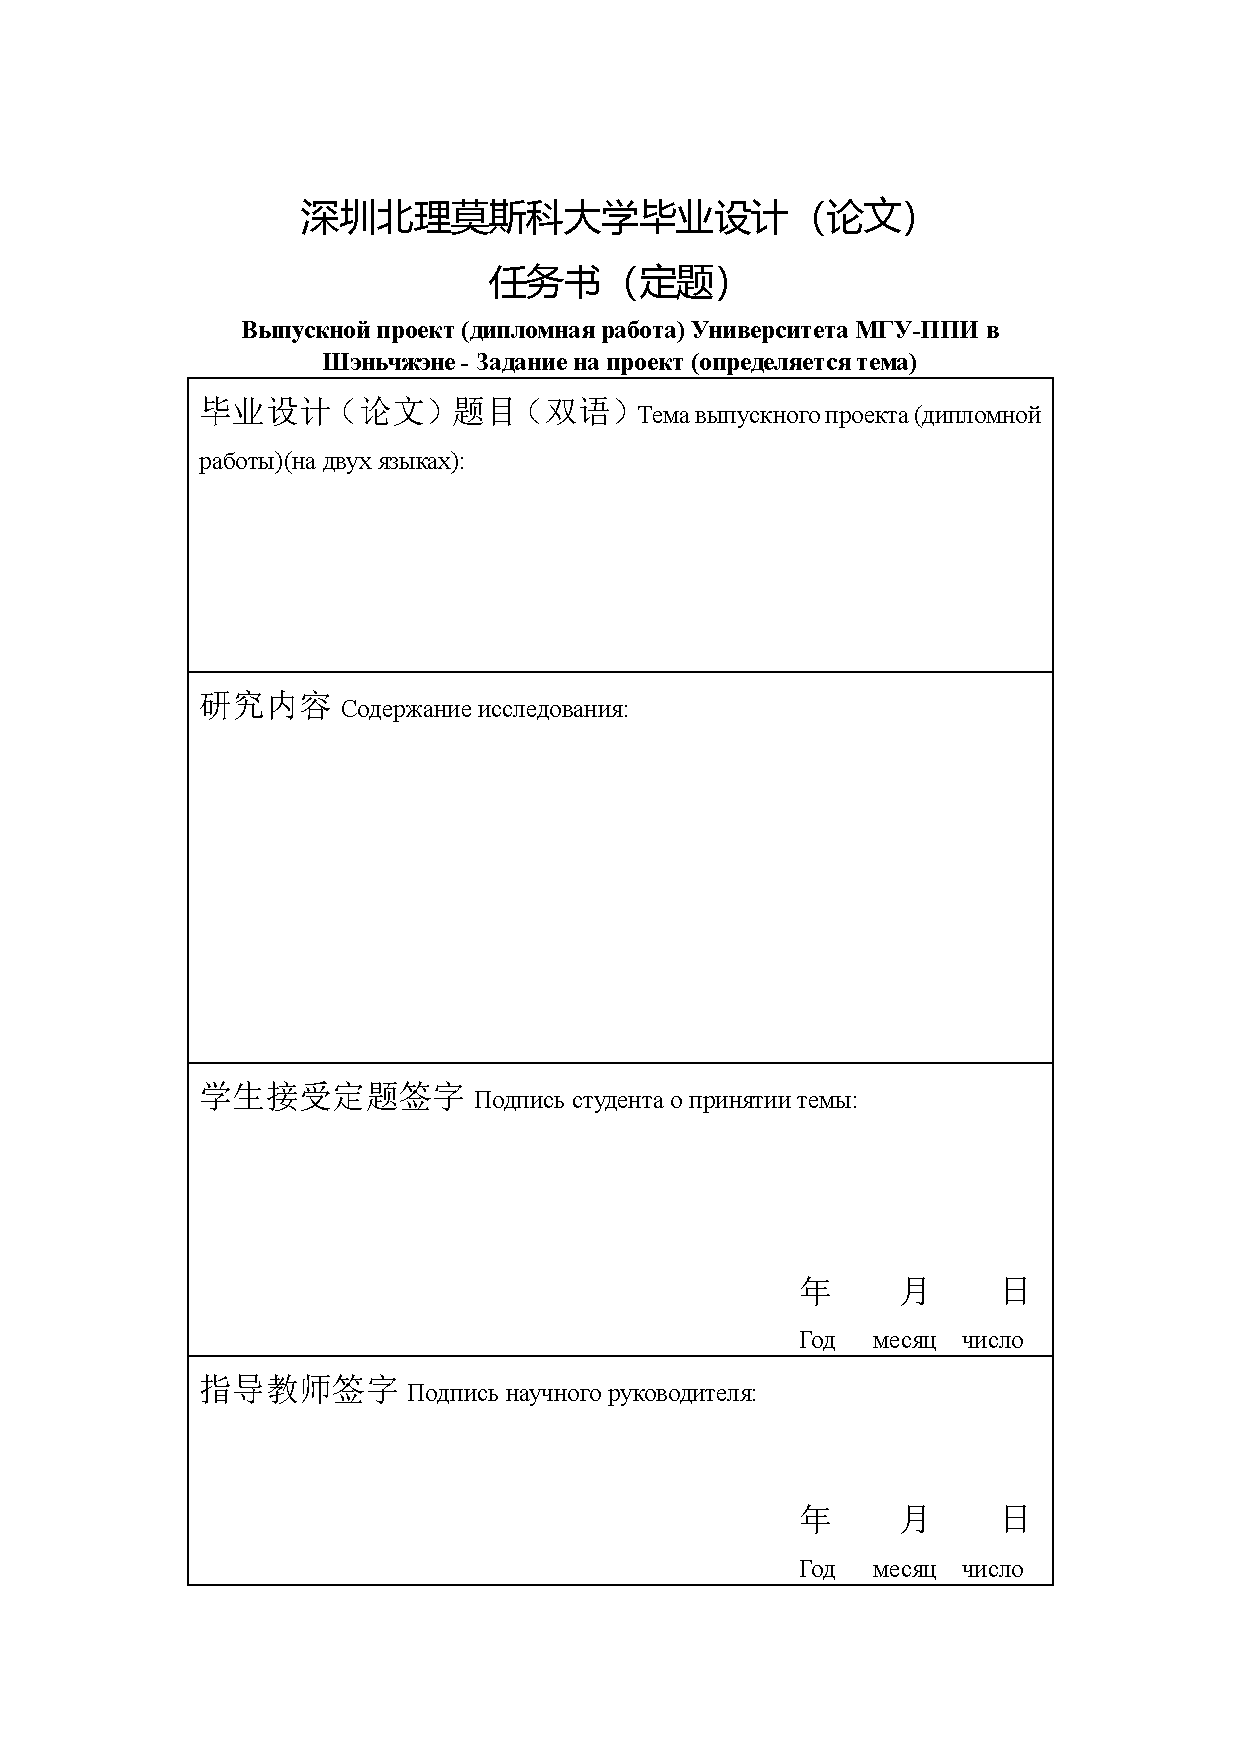
\includepdf[pages=1-5, pagecommand={\thispagestyle{fancy}}]{last.pdf}

\end{document}
